\documentclass[11pt]{article}
\usepackage[review]{acl}
\usepackage{times,latexsym,booktabs,amsmath,graphicx,xcolor,tikz}
\usepackage[T1]{fontenc}
\usetikzlibrary{arrows.meta}
\newcommand{\todo}[1]{\textcolor{red}{[TODO: #1]}}
\title{Two Clocks for Temporal Evidence Retrieval: \\ Valid Time versus Known Time in Versioned Official Documents}
\author{Anonymous ACL submission}
\begin{document}
\maketitle
\begin{abstract}
Temporal retrievers usually rank evidence by matching a query time against one document time or by preferring recent documents. Historical questions can constrain two different clocks, though: when a rule \emph{applied} (valid time) and when it could have been \emph{known} (publication time). The two disagree whenever a rule is announced before it takes effect, takes effect retroactively, expires, or is later corrected. We formalize a query as a target time $t$, an information horizon $h$ and an intent. We build a corpus of 3{,}650 Federal Register final rules in 405 recurring rule families, with effective dates verified against each rule's own text and end dates read from it. On 100 held-out families, single-clock rankers return evidence that is inadmissible under the requested semantics for 15 to 64\% of queries, and the best of them reaches 0.38 top-1. Routing each query to the matching clock, restricting candidates to rules in force and known at the stated times, and gating the candidate pool semantically reaches 0.80 with BM25 and 0.73 with a dense retriever. Blind LLM judges agree with our labels on 92\% of 120 cases drawn from the held-out families. \todo{human-annotated natural-language queries and agreement; real Re$^3$/Q-TIE comparison}
\end{abstract}

\section{Introduction}
Retrieval-augmented systems increasingly face questions about the past: which rule governed a transaction last year, or what an analyst could have known on a given date. Temporal retrievers and re-rankers such as Q-TIE~\cite{qtie2026} and Re$^3$~\cite{re32025} model when a query asks about and how recent a document should be. Q-TIE compares the query's interval with a document time; Re$^3$ separates a document's content time from its publication time. To our reading, neither treats the latest time at which evidence may be known as a constraint of the query.

In official sources a document has at least two relevant times. Consider the Consumer Financial Protection Bureau's annual Regulation Z threshold adjustments (Figure~\ref{fig:clocks}). The rule published on 1 August 2019 (Federal Register 2019-16300) takes effect on 1 January 2020, 153 days later. The rule it replaces (2018-18209) was published on 27 August 2018 and took effect on 1 January 2019. Asked on 1 November 2019, ``which threshold rule applied?'' has the 2018 rule as its answer, while ``which threshold rule could an analyst have found?'' has the 2019 rule. A ranker that prefers recent documents, or that cuts off by publication date, answers one question correctly and the other wrongly, and a validity filter does the reverse.

\begin{figure}[t]\centering
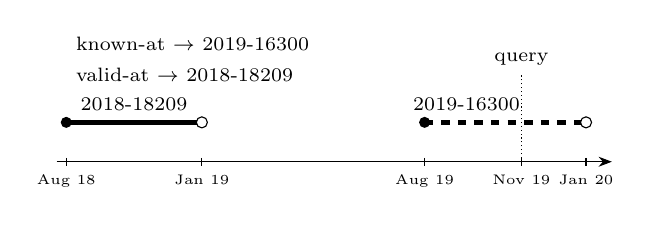
\begin{tikzpicture}[x=0.41cm,y=0.5cm,font=\scriptsize]
  \draw[-{Stealth}] (-0.3,0) -- (16.9,0);
  \foreach \x/\l in {0/{Aug 18},4.2/{Jan 19},11.1/{Aug 19},14.1/{Nov 19},16.1/{Jan 20}} {\draw (\x,0.1) -- (\x,-0.1); \node[below,font=\tiny] at (\x,-0.1) {\l};}
  \draw[line width=1.6pt] (0,1) -- (4.2,1); \fill (0,1) circle (2pt); \draw[fill=white] (4.2,1) circle (2pt);
  \node[above] at (2.1,1.05) {2018-18209};
  \draw[line width=1.6pt,dashed] (11.1,1) -- (16.1,1); \fill (11.1,1) circle (2pt); \draw[fill=white] (16.1,1) circle (2pt);
  \node[above] at (12.4,1.05) {2019-16300};
  \draw[densely dotted] (14.1,-0.1) -- (14.1,2.2); \node[above] at (14.1,2.2) {query};
  \node[anchor=west] at (0,2.2) {valid-at $\rightarrow$ 2018-18209};
  \node[anchor=west] at (0,3.0) {known-at $\rightarrow$ 2019-16300};
\end{tikzpicture}
\caption{Two clocks on one rule family (Regulation Z annual threshold adjustments). Each bar runs from publication (filled dot) to effective date (open dot). The query is dated 1 November 2019 ($t{=}h$) and has a different correct answer under each intent: the 2018 rule is the one in force, the 2019 rule is the latest one published.}\label{fig:clocks}
\end{figure}

Making the right choice poses three challenges. The system must infer from natural language which clock a query constrains. Versions of one rule often share most of their text, so semantic relevance alone separates them poorly and must be combined with time, without letting time pull in unrelated documents. And effective dates are sometimes missing or unreliable. We address these with an intent router, hard eligibility under the requested semantics, and a semantic gate on the candidate pool. The distinction between valid and transaction time is classical~\cite{jensen1996}, has been argued for legal retrieval~\cite{demartim2026}, and appears as a filter in agent memory stores~\cite{niksarli2026}. We found no measurement of how single-clock rankers fail on versioned authoritative documents, and no query formulation that makes the choice of clock explicit.

We contribute (i) the $(t,h,\text{intent})$ formulation (Section~\ref{sec:form}); (ii) a verified real-world corpus and probe protocol (Section~\ref{sec:data}); (iii) a comparison of single-clock baselines with intent-routed two-clock eligibility (Sections~\ref{sec:method} and~\ref{sec:exp}); and (iv) an analysis of missing timestamps, corrections and harm to ordinary queries (Section~\ref{sec:exp}).

\section{Related Work}
\textbf{Temporal retrieval.} Q-TIE maps a query's temporal constraint to an interval and re-ranks against document time~\cite{qtie2026}. Re$^3$ is the closest to our setting: it describes a document by a content (clue) time and a publication time and learns a gate over relevance, temporal alignment and freshness~\cite{re32025}. MRAG decomposes time-sensitive questions with constraints such as ``as of'' and judges evidence by temporal reasoning~\cite{mrag2025}, and TEMPS adds an anchor-date temporal score to dense retrievers~\cite{temps2026}. IA-RAG represents facts as intervals related by Allen's algebra~\cite{iarag2026}. FRESCO and HoH study evolving or outdated documents in the retrieval pool~\cite{fresco2026,hoh2025}, and TimelyRAG reranks over overlapping, evolving documents~\cite{timelyrag2026}. TEMPO evaluates whether retrieved evidence covers the time periods a query needs~\cite{tempo2026}. In the papers we read, none states the latest time at which evidence may be known as a constraint on the query, or measures how often returned evidence violates such a constraint.

\textbf{Bitemporal modeling.} Valid and transaction time are standard in temporal databases~\cite{jensen1996}. Recent work applies them to legal retrieval as a design argument~\cite{demartim2026} and to agent memory as a storage and filter mechanism~\cite{niksarli2026}. We study what they mean for ranking on a versioned document collection.

\section{Problem Formulation}\label{sec:form}
A query has a target time $t$, an information horizon $h$ (the latest time at which evidence may be known) and an intent. A document $d$ has a publication time $p_d$, which we use as a proxy for when it became known, an effective time $e_d$ (valid-from), and, where the document states one, an end of validity $v_d$ ($v_d=\infty$ otherwise). The document is \emph{in force} at $t$ if $e_d\le t\le v_d$. We define four intents, each with a single best version as gold. \emph{Current}: the latest document in force today ($\tau$) with $p_d\le\tau$. \emph{Valid-at}: the latest in force at $t$, with later publication allowed. \emph{Known-at}: the latest with $p_d\le h$. \emph{Valid-known}: the latest in force at $t$ with $p_d\le h$. Notices that only correct, withdraw or postpone another rule are not versions of their own, and ties between rules with the same date go to the later publication, then the higher document number. If no document qualifies, the correct answer is \textsc{none}, and a system should abstain. A returned document is \emph{inadmissible} if it violates the constraints of the intent. Correction notices are evaluated separately. A correction is published at $p_k>p_0$, where $p_0$ is the original's publication time. A known-at query with $h<p_k$ requires the original, and a retrospective query ($h=\tau$) requires the corrected record.

\section{Data}\label{sec:data}
We collect Federal Register final rules from 2010 to 2026 (US government works; reuse terms to be confirmed before release), drawn from 84 CFR parts and, for the later batches, whole CFR titles. A family is a set of documents with the same digit-masked title and at least four versions across at least three years. It must also contain either two rules whose effective date is at least 14 days after publication or one retroactive rule; the first mining pass used only the first condition. The corpus has 3{,}650 rules in 405 families and 5{,}247 probe cases. Each case is placed between a rule's publication and effective date (between effective and publication for retroactive rules), so the clocks disagree by construction. Every effective date appears verbatim in the rule's DATES text (3{,}649 of 3{,}650; four rules whose API date conflicts with their own text were excluded). We read $v_d$ from the same statement (``through'', ``until'', a from--to window, or a time-of-day window on one date) and find an end date for 2{,}025 rules.

Splits are by family. Selection used 9 dev and 56 dev2 families. Five batches of held-out families were frozen before use: 5 and 35 families (\texttt{test1}, \texttt{test2}), and three fresh batches of 100 families each (\texttt{test3}, \texttt{test4}, \texttt{test5}). The end-of-validity semantics were introduced after a judging check on \texttt{test3} and \texttt{test4}, and their remaining rules (time windows, notices, tie-breaks) were designed on a separate dev sample (Section~\ref{sec:judge}), so \texttt{test5}, drawn from families never used before, is the clean test for the final semantics. \todo{human-written natural-language queries and relevance judgments, inter-annotator agreement}

\section{Method}\label{sec:method}
\textbf{Router.} A cue-based router maps a query to an intent: date-free queries go to current, knowledge cues without validity cues to known-at, validity plus restriction cues to valid-known, and everything else to valid-at. A regex parser extracts $t$ and $h$. \textbf{Eligibility.} We keep the candidates $E$ that satisfy the intent's constraints, using the in-force interval $[e_d, v_d]$. If $E$ is empty the system abstains. \textbf{Ranking.} Let $z_d$ be the $z$-scored semantic score of $d$ within the candidate pool and $g_d$ the gap in days between the intent's reference time and $d$'s time on the intent's clock. V1 ranks $E$ by
\begin{equation}\label{eq:v1}
s_1(d) = z_d - \lambda \log\!\left(1 + g_d/30\right),
\end{equation}
with $\lambda$ chosen on dev. V2 first applies a semantic gate and then orders by temporal gap:
\begin{equation}\label{eq:v2}
\begin{split}
\mathcal{G} &= \{d \in E : z_d \ge \max_{d'} z_{d'} - \delta\},\\
&\text{rank } \mathcal{G} \text{ by } (g_d,\,-z_d),
\end{split}
\end{equation}
where the maximum is taken over the whole pool, not only $E$. The pool holds the top 50 documents by BM25 or by cosine similarity of a small embedding model; the pool size and $\delta$ were chosen on dev. A candidate with a missing effective date is dropped (the system abstains) instead of being imputed from its publication time.

\section{Experiments}\label{sec:exp}
\textbf{Baselines.} B0 is plain retrieval. B2 is a publication cutoff at $h$, and B3 a validity-interval filter at $t$. B6 is a soft temporal distance on publication date, a TimelyRAG-style approximation and not a reproduction. We also built a Q-TIE-style point-interval scorer and a Re$^3$-style relevance and recency gate; both are approximations from the papers' descriptions, because the official Q-TIE code was unavailable and we found no released Re$^3$ code. A one-sided-interval method with a single document clock is bounded by B2 and B3. We use BM25 and, to check that the result is not specific to lexical matching, a small embedding model (bge-small-en-v1.5).

\begin{table}[t]\centering\small
\begin{tabular}{lcccc}\toprule
 & \multicolumn{2}{c}{BM25} & \multicolumn{2}{c}{Dense} \\
Method & top-1 & inadm. & top-1 & inadm. \\\midrule
B0 retrieval & .19 & .63 & .10 & .71 \\
B2 pub.\ cutoff & .17 & .61 & .16 & .59 \\
B3 validity filter & .27 & .17 & .19 & .16 \\
B6 soft dist.\ & .32 & .61 & .32 & .60 \\
B4 v1 ($\lambda{=}2$) & .57 & .00 & .49 & .00 \\
B4 v2 ($\delta{=}1.5$) & \textbf{.80} & .00 & \textbf{.73} & .00 \\\bottomrule
\end{tabular}
\caption{Top-1 accuracy and rate of inadmissible top results on the clean held-out batch (\texttt{test5}: 100 families, 1{,}252 cases; abstention counts as correct only when no rule qualifies). Pool 50 for BM25 and pool 100 for the dense scorer, both chosen on dev; B3 reaches .38 with a pool of 20. By intent, v2 with BM25 scores .78 (current), .81 (valid-at), .84 (known-at) and .75 (valid-known).}\label{tab:main}
\end{table}

\textbf{Main result.} Each single-clock baseline fails on the intent it does not model (with BM25, B2 reaches 0.00 on valid-at and B3 0.01 on known-at). Against the best pool size for each baseline, v2 improves overall top-1 by 0.42 over B3, 0.47 over B6 and 0.58 over B2 (family-cluster bootstrap on 100 families: $+.42$ [.36,.48], $+.47$ [.38,.55], $+.58$ [.50,.66]); with a dense retriever, $+.54$ [.46,.62] over B3. The semantic gate adds $+.23$ [.17,.30] over $\lambda$-weighting at pool 50. Before end dates were modeled, the same configuration reached 0.70 (pool 20) and 0.79 (pool 50) on two other fresh batches (\texttt{test3}, \texttt{test4}) against at most 0.35 for the single-clock baselines.

\begin{table}[t]\centering\small
\begin{tabular}{lcc}\toprule
Variant & top-1 & inadm. \\\midrule
Full v2 & .80 & .00 \\
$-$ routing (always valid-at) & .50 & .15 \\
$-$ routing (always known-at) & .27 & .63 \\
$-$ eligibility (gate and gap only) & .07 & .91 \\
$-$ semantic gate (eligibility and gap) & .45 & .00 \\\bottomrule
\end{tabular}
\caption{Ablation of v2 with BM25 on \texttt{test5} (1{,}252 cases) with the frozen configuration. Removing routing, eligibility or the gate each lowers top-1; eligibility carries the most.}\label{tab:abl}
\end{table}

\textbf{Ablation.} Table~\ref{tab:abl} isolates each component. Without eligibility, top-1 falls to 0.07 and 91\% of top results are inadmissible. Fixing one intent for every query gives 0.50 or 0.27, so routing matters as well. Dropping the semantic gate costs 0.35.

\subsection{Independent check with blind judges}\label{sec:judge}
Our labels come from the same dates the method uses, so we checked them against readers who never saw our metadata. Six LLM judges (Claude Sonnet) received plain-language questions and, for every candidate rule, its publication date and its own DATES statement, but no formal definitions and no intent labels, and picked the best rule or \textsc{none}. These are machine judges, not human annotators.

On a first sample of 120 cases from \texttt{test3} and \texttt{test4}, agreement with our original labels was 0.74 (valid-known 0.43). Twenty-three judge answers were \textsc{none}, which the original labels never allowed, and most disagreements involved rules that had already expired. We then added end-of-validity semantics, and extended the date reader to from--to windows after reading four DATES statements from that sample; agreement on the same sample rose to 0.93. We judged a second, development sample of 120 cases from dev families: agreement was 0.92, and fixes designed on it (time-of-day windows, notices that only correct or postpone another rule, deterministic tie-breaks) raised it to 0.95. On 120 cases from \texttt{test5}, which no choice had used, agreement was 106 of 120 (0.88) before those fixes and 110 of 120 (0.92) after them: known-at 1.00, current 0.93, valid-at 0.87, valid-known 0.87. The remaining disagreements involve rules delayed or partly postponed by later notices, ``effective without actual notice'' statements, and ties. \todo{replace or complement with human annotation}

\textbf{Corrections.} On 106 correction chains (212 cases; earlier semantics, pool 20), a cutoff at the target time returns the superseded original for every retrospective query (top-1 0.00). A cutoff at the routed horizon with the semantic gate reaches 0.87 on retrospective queries and 0.99 on known-at queries.

\textbf{Missing dates.} In the same earlier setting, hiding 30\% of effective dates lowers top-1 from 0.87 to 0.71 and produces no inadmissible results when candidates are dropped. Imputing effective time from publication time adds 1 to 10 points of top-1 but returns inadmissible evidence for 5 to 55\% of queries.

\textbf{Ordinary queries.} Applying a temporal rule to every topic-only query drops nDCG@10 from 0.98 to 0.46. Routing with the gate keeps it at 0.92.

\section{Conclusion}
Historical evidence questions constrain either when a rule applied, when it could have been known, or both, and a rule can also have expired or have no valid answer at all. On versioned Federal Register rules, rankers that use one clock fail on the other intent. Routing each query to the matching clock, requiring evidence to be in force and known at the stated times, and gating the candidate pool semantically removes the inadmissible results and reaches 0.80 top-1 with BM25 and 0.73 with a dense retriever on a clean batch of 100 families. A blind-judge check agrees with our labels on 92\% of cases. The next steps are human-judged relevance on independently written queries and a comparison with the official Re$^3$ and Q-TIE systems.

\section{Limitations}
Our labels come from the same dates that eligibility uses, so inadmissibility is zero by construction and relevance is single-gold; the judge check agrees on 92\% of cases but the judges are language models, not human annotators, and may share biases with the system builder's assistant. Human-annotated, independently written queries and relevance judgments have not been reported. The end-of-validity reader mis-parses some statements, does not link delay or confirmation notices to the rules they modify, and treats ties between rules with the same date by a fixed convention. We evaluate BM25 and one small embedding model; larger retrievers and cross-encoders are untested. Publication time is only a proxy for knowledge time, and all data come from one jurisdiction and document type. The intent router and date parser were developed on author-written queries. Q-TIE and Re$^3$ are approximated, not reproduced. The pool size and gate width were chosen on dev after an error analysis, and the semantic-gate variant was designed after inspecting aggregate error categories on earlier splits. Random timestamp masking does not model systematic missingness.

\section*{Ethics Statement}
The corpus consists of public-domain US government rules and contains no personal data. Reuse terms for any released resource should be confirmed.

\bibliography{references}
\end{document}
